\begin{frame}<1>[label=rbInsertCases]{red-black insert}
\begin{itemize}
\item default: insert as \nred{red}, but\ldots
\item \myemph<2>{(1) if new node is root}: color \nblack{black}
\item \myemph<3>{(2) if parent is black}: keep child \nred{red}
\item \myemph<4>{(3) if parent and uncle is \nred{red}}: adjust several colors
\item \myemph<5>{(4) if parent is \nred{red}, uncle is \nblack{black}}, new node is right child
    \begin{itemize}
    \item perform a rotation, then go to case 5
    \end{itemize}
\item \myemph<6>{(5) if parent is \nred{red}, uncle is \nblack{black}}, new node is left child
    \begin{itemize}
    \item perform a rotation
    \end{itemize}
\end{itemize}
\begin{tikzpicture}[overlay, remember picture]
\coordinate (where) at ([yshift=1cm]current page.south);
\tikzset{
    box/.style={draw,very thick,fill=white,at=(where), anchor=south, align=left},
}
\begin{visibleenv}<2>
\node[box] {
    property: ``root is black'' \\
    no children $\rightarrow$ no worries about \# black nodes \\
    on different paths
};
\end{visibleenv}
\begin{visibleenv}<3>
\node[box] {
    property: ``children of \nred{red} node are \nblack{black}'' \\
    no change in \# of \nblack{black} nodes on paths 
};
\end{visibleenv}
\end{tikzpicture}
\end{frame}

\againframe<3>{rbInsertCases}

\againframe<4>{rbInsertCases}

\begin{frame}{case 3: parent, uncle are red}
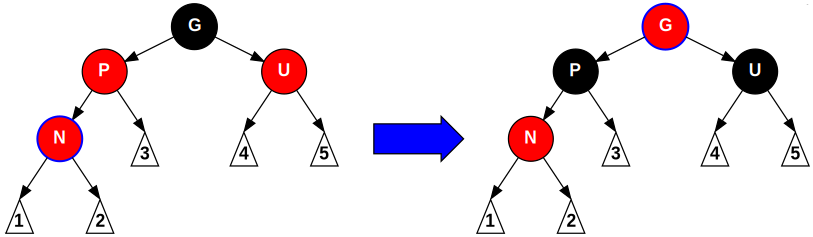
\includegraphics[width=0.9\textwidth]{Red-black_tree_insert_case_3}
\begin{itemize}
\item make grandparent \nred{red}, parent and uncle \nblack{black}
    \begin{itemize}
    \item (property: every path to leaf has same number of black nodes)
    \item just swapped grandparent and parent/uncle in those paths
    \end{itemize}
\item<2-> but\ldots what if grandparent's parent is red?
    \begin{itemize}
    \item (property: children of red node are black)
    \item solution: \myemph<3>{recurse to the grandparent}, as if it was just inserted
    \end{itemize}
\end{itemize}
\end{frame}

\againframe<5>{rbInsertCases}

\begin{frame}{case 4: parent red, uncle black, right child}
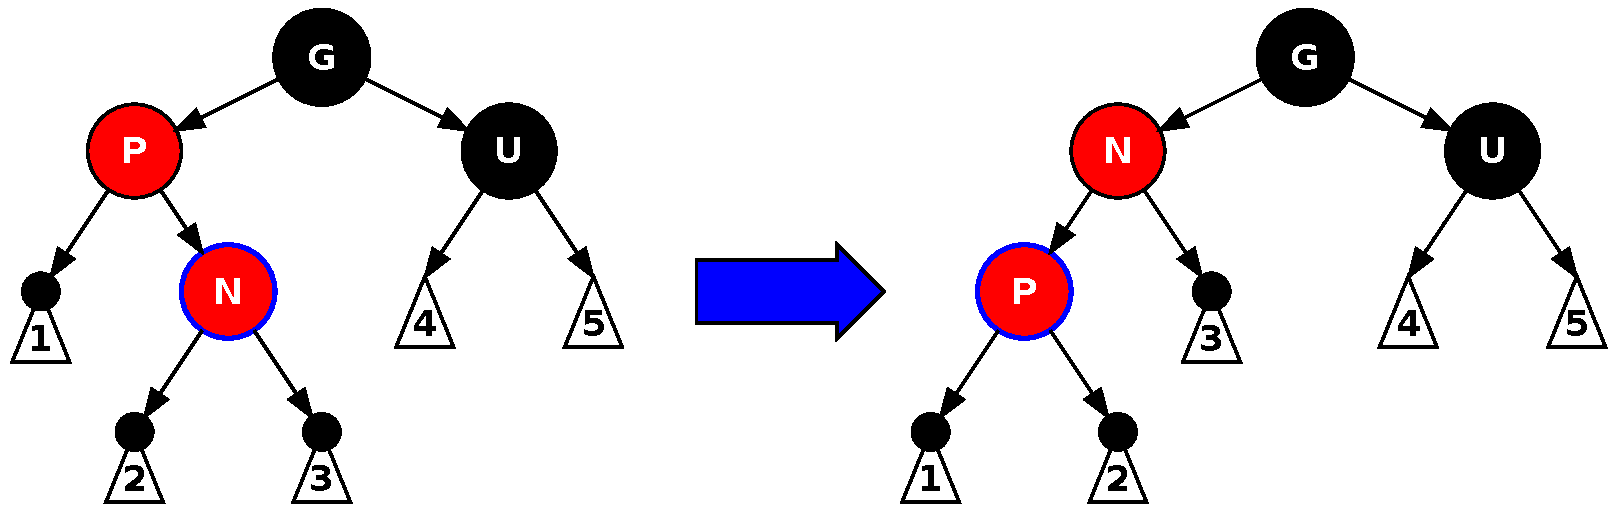
\includegraphics[width=0.9\textwidth]{Red-black_tree_insert_case_4}
\begin{itemize}
\item perform left rotation on parent subtree and new node
\item now case 5 (but new node is $P$, not $N$)
\end{itemize}
\end{frame}

\againframe<6>{rbInsertCases}

\begin{frame}{case 5: parent red, uncle black, left child}
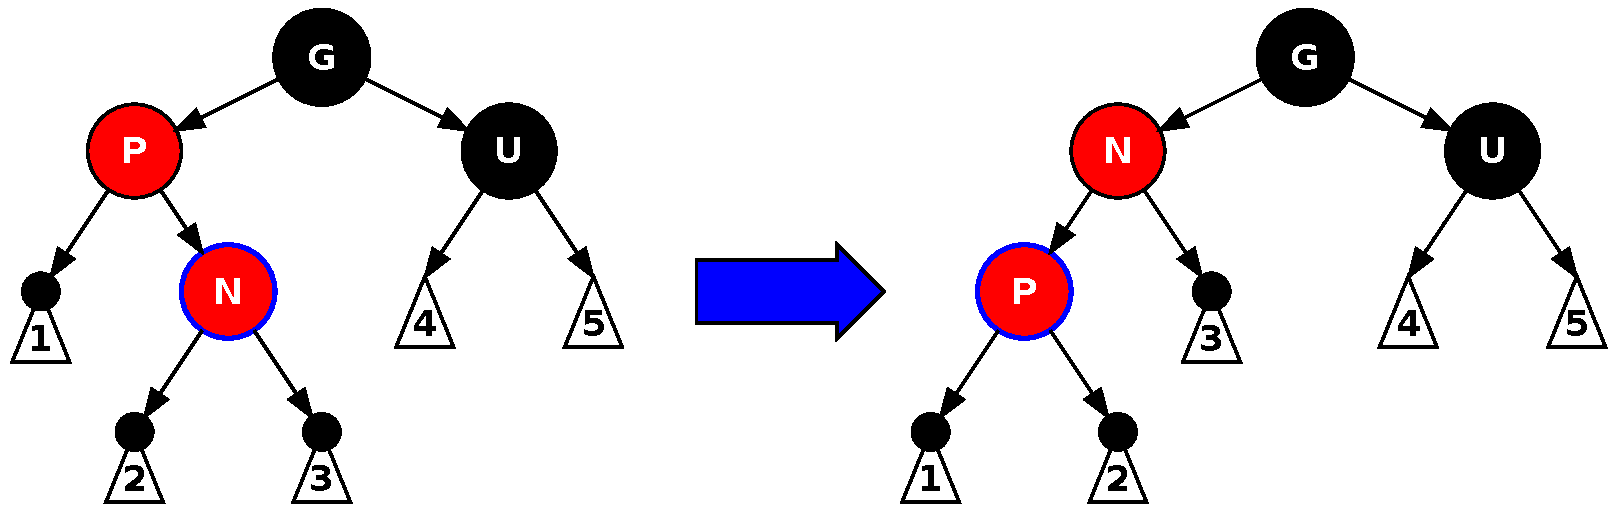
\includegraphics[width=0.9\textwidth]{Red-black_tree_insert_case_4}
\begin{itemize}
\item perform right rotation of grandparent and parent
\begin{itemize}
    \item (property: red parent's children are black)
    \item (property: every path to leaf has same number of black nodes)
\end{itemize}
\end{itemize}
\end{frame}
